% Chapter 11: genome-wide association studies.
% Requires: amsmath, amssymb, bm, graphicx, booktabs, subcaption,
% tikz (arrows.meta, positioning, calc, decorations.pathreplacing, fit), natbib.
% Computed figures are produced by scripts/make_figures.py; figures/slides/ holds figures taken from the lecture slides.

\providecommand{\R}{\mathbb{R}}
\providecommand{\E}{\mathbb{E}}
\providecommand{\Normal}{\mathcal{N}}
\providecommand{\argmax}{\operatorname*{arg\,max}}
\providecommand{\argmin}{\operatorname*{arg\,min}}
\providecommand{\vy}{\mathbf{y}}
\providecommand{\vx}{\mathbf{x}}
\providecommand{\mX}{\mathbf{X}}
\providecommand{\mI}{\mathbf{I}}
\providecommand{\vb}{\boldsymbol{\beta}}
\providecommand{\veps}{\boldsymbol{\epsilon}}
\providecommand{\vp}{\mathbf{p}}
\providecommand{\vg}{\mathbf{g}}
\providecommand{\ind}{\mathbf{1}}
\providecommand{\vz}{\mathbf{z}}
\providecommand{\vzh}{\hat{\mathbf{z}}}
\providecommand{\ve}{\mathbf{e}}
\providecommand{\vu}{\mathbf{u}}
\providecommand{\vr}{\mathbf{r}}
\providecommand{\va}{\mathbf{a}}
\providecommand{\vc}{\mathbf{c}}
\providecommand{\vone}{\mathbf{1}}
\providecommand{\vgamma}{\boldsymbol{\gamma}}
\providecommand{\vtheta}{\boldsymbol{\theta}}
\providecommand{\vlambda}{\boldsymbol{\lambda}}
\providecommand{\mR}{\mathbf{R}}
\providecommand{\mK}{\mathbf{K}}
\providecommand{\mU}{\mathbf{U}}
\providecommand{\mS}{\mathbf{S}}
\providecommand{\mC}{\mathbf{C}}
\providecommand{\mA}{\mathbf{A}}
\providecommand{\mH}{\mathbf{H}}
\providecommand{\mZ}{\mathbf{Z}}
\providecommand{\Var}{\operatorname{Var}}
\providecommand{\Cov}{\operatorname{Cov}}
\providecommand{\logit}{\operatorname{logit}}

\chapter{Genome-wide association studies}
\label{ch:gwas}

So far this book has mostly modelled molecular measurements of cells: expression, chromatin accessibility, transcription factor binding, methylation. This chapter turns to the other main use of sequencing introduced in Chapter 1, reading the genomes of many individuals and relating the differences between them to traits and diseases. A genome-wide association study (GWAS) tests each of millions of genetic variants for association with a trait. Statistically, a GWAS is little more than millions of small linear or logistic regressions, but it has to deal with three complications that make it interesting from a machine learning point of view: the features (genotypes) are strongly correlated with their neighbours along the genome, the samples (people) are not independent because they share ancestry, and the effects are tiny and numerous. We first describe human genetic variation and how a GWAS is run, then the population genetics that creates correlation between variants, then the statistical tools built on top of GWAS results: linear mixed models for population structure, summary statistics, fine-mapping and LD score regression. We end with an example where the biology of a GWAS association was worked out in detail, the obesity association at the \textit{FTO} locus.

%======================================================================
\section{Human genetic variation}
\label{sec:variation}
%======================================================================

Humans are diploid: apart from the sex chromosomes, each person carries two copies of every chromosome, one inherited from each parent. The human genome is about $3\times10^9$ base pairs (bp) long and contains roughly 20{,}000--25{,}000 protein-coding genes. Two copies of the genome, whether the two copies within one person or copies from two different people, differ at roughly one position in every thousand. A typical genome differs from the reference genome at 4--5 million sites~\citep{kg2015}. Almost all of these differences are inherited; a few dozen per person (of the order of 50--100) are \emph{de novo} mutations that arose in a parent's egg or sperm.

A position where the population carries more than one nucleotide is \emph{polymorphic}. The alternative versions are called \emph{alleles}. Most polymorphic positions are \emph{bi-allelic}, with two alleles. Genetic variants are classified by size:
\begin{itemize}
  \item \emph{Single nucleotide polymorphisms} (SNPs) change one nucleotide. There are about 3 million \emph{common} SNPs, conventionally those whose rarer allele has frequency above 5\% in a population, and many more rare ones, down to \emph{private} variants seen in one family and \emph{de novo} variants seen in one person.
  \item \emph{Indels} are short insertions or deletions, up to about 50 bp.
  \item \emph{Structural variants} are larger insertions, deletions (\emph{copy number variants}), inversions and other rearrangements, up to millions of bp.
\end{itemize}
All of these are \emph{germline} variants, present in every cell and passed on to children. \emph{Somatic} mutations arise in a single cell during a person's lifetime, by chance or through exposures such as tobacco smoke or ultraviolet light, and are inherited only by that cell's descendants. They drive cancer but are not the subject of this chapter.

At a bi-allelic SNP we call the allele in the human reference genome the \emph{reference} allele and the other the \emph{alternative} allele. The rarer of the two in a population is the \emph{minor} allele, and its frequency is the \emph{minor allele frequency} (MAF), at most $0.5$. A person's \emph{genotype} at the SNP is the unordered pair of alleles they carry, for example AA, AC or CC. We usually ignore which allele came from which parent. (The exception is \emph{imprinting}, where only the copy from one parent is expressed.)

Most SNPs are rare. Under the simplest population genetic model, a population of constant size with no selection, the expected number of SNPs at which the alternative allele is carried by $i$ of $n$ sampled chromosomes is proportional to $1/i$. Rare variants therefore make up most SNPs (Figure~\ref{fig:sfs}, blue). Real human populations have grown rapidly in the last few thousand years, which adds still more rare variants. Rare variants contribute little to the differences between two people, however. A person is heterozygous at a SNP with allele frequency $f$ with probability $2f(1-f)$, so most of the sites at which one person carries two different alleles are common SNPs (Figure~\ref{fig:sfs}, orange).

\begin{figure}[!htbp]
  \centering
  \includegraphics[width=0.75\linewidth]{sfs.pdf}
  \caption{Expected allele frequency distribution under the neutral constant-size model, for a sample of 20{,}000 chromosomes. Blue, the share of all SNPs in each minor allele frequency bin: most SNPs are rare. Orange, the share of the heterozygous sites of one individual: these are mostly common SNPs.}
  \label{fig:sfs}
\end{figure}

%======================================================================
\section{Why look for the genetic basis of disease?}
%======================================================================

There are three main motivations for mapping the genetic variants that affect disease risk.
\begin{enumerate}
  \item \emph{Understanding disease biology.} Complex diseases are often studied in animal models, for example mice engineered to carry human risk genes. These models reproduce some aspects of a human disease but not others. A mouse lives about two years, so a mouse model of a late-onset disease such as Alzheimer's disease has neurons that are two years old rather than seventy. Genetic associations come from human data, so they point at processes that matter in the human disease.
  \item \emph{Personalized prediction and treatment.} If we knew the variants that affect risk we could predict who is at higher risk and intervene earlier. This works well for some variants with large effects; for most common diseases, prediction from genotype remains modest.
  \item \emph{Identifying drug targets.} Retrospective analyses of drug development pipelines found that drug targets supported by human genetic evidence are about twice as likely to progress from clinical trials to approval~\citep{nelson2015,king2019} (Chapter 1). Given that bringing one drug to market costs of the order of a billion dollars, this is a strong argument for genetics.
\end{enumerate}

%======================================================================
\section{Mendelian and complex traits}
%======================================================================

\subsection{Mendelian genetics}

The first well-understood genetics was Gregor Mendel's work on pea plants~\citep{mendel1866}, decades before DNA was known to carry hereditary information. Consider one position in the genome with two alleles, A and T, and two parents that are both heterozygous, AT (Figure~\ref{fig:punnett}). Each gamete (pollen grain or egg cell in the plant, sperm or egg in a human) carries one copy of the genome, and so one of the parent's two alleles, chosen with probability $1/2$ each. Which gametes combine is also random, so an offspring is AA, AT or TT with probabilities $1/4$, $1/2$ and $1/4$.

In Mendel's flowers the A allele is \emph{dominant}: one copy is enough to make the flower purple, and only TT plants are white. The T allele is \emph{recessive}. A biochemical explanation could be that the T allele breaks an enzyme that makes purple pigment, and a single working copy of the enzyme makes enough pigment.

\begin{figure}[!htbp]
  \centering
  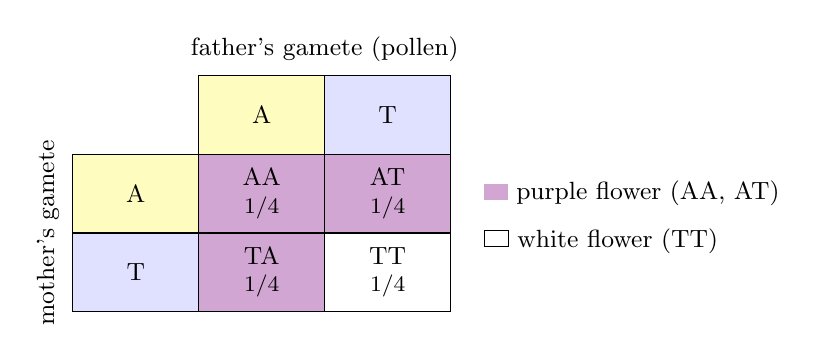
\begin{tikzpicture}[every node/.style={font=\small}, cell/.style={minimum width=1.6cm, minimum height=1.0cm, draw, align=center}]
    \node[cell, fill=yellow!25] at (1.6,1.0) {A};
    \node[cell, fill=blue!12] at (3.2,1.0) {T};
    \node[cell, fill=yellow!25] at (0,0) {A};
    \node[cell, fill=blue!12] at (0,-1.0) {T};
    \node[cell, fill=violet!35] at (1.6,0) {AA\\[-1pt]\footnotesize $1/4$};
    \node[cell, fill=violet!35] at (3.2,0) {AT\\[-1pt]\footnotesize $1/4$};
    \node[cell, fill=violet!35] at (1.6,-1.0) {TA\\[-1pt]\footnotesize $1/4$};
    \node[cell, fill=white] at (3.2,-1.0) {TT\\[-1pt]\footnotesize $1/4$};
    \node[above] at (2.4,1.55) {father's gamete (pollen)};
    \node[rotate=90, above] at (-0.85,-0.5) {mother's gamete};
    \node[right, align=left] at (4.3,0.0) {\tikz\fill[violet!35] (0,0) rectangle (0.3,0.2); purple flower (AA, AT)};
    \node[right, align=left] at (4.3,-0.6) {\tikz\draw (0,0) rectangle (0.3,0.2); white flower (TT)};
  \end{tikzpicture}
  \caption{A Punnett square for a cross between two heterozygous (AT) parents. Each gamete carries one allele, chosen at random, so each of the four combinations has probability $1/4$. With A dominant, three quarters of the offspring have the dominant (purple) phenotype.}
  \label{fig:punnett}
\end{figure}

Many human diseases follow this pattern. They are called \emph{Mendelian} diseases because a variant in a single gene is enough to cause them. Cystic fibrosis is a recessive disease caused by loss-of-function variants in \textit{CFTR}, which encodes a chloride channel~\citep{riordan1989}. It is the most common severe recessive disease in people of European ancestry, about 4\% of whom are heterozygous \emph{carriers}. Carriers are healthy, because one working copy suffices, but each child of two carriers has a $1/4$ chance of inheriting two broken copies, exactly as for the white flower. Marriage between relatives raises the probability that both parents carry the same rare recessive variant, inherited from a shared ancestor. Mendelian disease genes were mapped by following variants through families and are catalogued in Online Mendelian Inheritance in Man (OMIM).

\subsection{Complex traits}

Most common diseases, such as type 2 diabetes, schizophrenia and Alzheimer's disease, and quantitative traits such as height do not follow Mendelian patterns. They are called \emph{complex} traits. For these~\citep{manolio2009}:
\begin{itemize}
  \item no single variant is necessary or sufficient for disease;
  \item many genes and variants contribute, each with a small effect on risk, often raising it by a few percent;
  \item environment and chance also matter: diet and exercise for type 2 diabetes, for example;
  \item a single diagnosis can cover heterogeneous underlying mechanisms. Alzheimer's disease includes forms dominated by memory loss and forms dominated by language impairment, and neurodevelopmental conditions such as autism vary widely within a diagnosis;
  \item rare variants, \emph{de novo} mutations, interactions between variants (\emph{epistasis}) and parent-of-origin effects may contribute. Even the largest current studies are too small to test interactions between variants systematically, so most analyses assume that effects add up across the genome.
\end{itemize}
There are also indirect effects. Parents' genotypes affect their children's traits beyond the alleles the children inherit, for example through the environment the parents provide; this is sometimes called \emph{genetic nurture}~\citep{kong2018}.

Genome-wide association studies were designed for complex traits. The number of genome-wide significant associations has grown from a handful in 2006 to hundreds of thousands, catalogued in the GWAS Catalog~\citep{buniello2019}.

%======================================================================
\section{The genome-wide association study}
\label{sec:gwas_model}
%======================================================================

\subsection{Case-control association}

The simplest GWAS compares people who have a disease (\emph{cases}) with people who do not (\emph{controls}). Controls should be matched to cases on factors such as age: for a late-onset disease such as Alzheimer's, a young control may simply not have developed the disease yet. Each person is genotyped, traditionally with a genotyping array that measures a few hundred thousand chosen SNPs and increasingly by whole-genome sequencing. At each SNP we tabulate genotype counts in cases and controls and test whether genotype and disease status are independent (Figure~\ref{fig:casecontrol}).

\begin{figure}[!htbp]
  \centering
  \begin{tikzpicture}[every node/.style={font=\small}, >=Stealth]
    \node[anchor=west, inner sep=0] at (0,0.00) {\texttt{GGCATACG\textcolor{orange!80!black}{\textbf{A}}TATTAGCAA\textcolor{green!45!black}{\textbf{A}}TAAAC}};
    \node[anchor=west, inner sep=0] at (0,-0.42) {\texttt{GGCATACG\textcolor{orange!80!black}{\textbf{A}}TATTAGCAA\textcolor{green!45!black}{\textbf{A}}TAAAC}};
    \node[anchor=west, inner sep=0] at (0,-0.84) {\texttt{GGCATACG\textcolor{orange!80!black}{\textbf{A}}TATTAGCAA\textcolor{green!45!black}{\textbf{A}}TAAAC}};
    \node[anchor=west, inner sep=0] at (0,-1.26) {\texttt{GGCATACG\textcolor{orange!80!black}{\textbf{C}}TATTAGCAA\textcolor{green!45!black}{\textbf{G}}TAAAC}};
    \node[anchor=west, inner sep=0] at (0,-1.68) {\texttt{GGCATACG\textcolor{orange!80!black}{\textbf{C}}TATTAGCAA\textcolor{green!45!black}{\textbf{G}}TAAAC}};
    \node[anchor=west, inner sep=0] at (0,-2.10) {\texttt{GGCATACG\textcolor{orange!80!black}{\textbf{A}}TATTAGCAA\textcolor{green!45!black}{\textbf{A}}TAAAC}};
    \node[anchor=west, inner sep=0] at (0,-2.87) {\texttt{GGCATACG\textcolor{orange!80!black}{\textbf{A}}TATTAGCAA\textcolor{green!45!black}{\textbf{A}}TAAAC}};
    \node[anchor=west, inner sep=0] at (0,-3.29) {\texttt{GGCATACG\textcolor{orange!80!black}{\textbf{C}}TATTAGCAA\textcolor{green!45!black}{\textbf{G}}TAAAC}};
    \node[anchor=west, inner sep=0] at (0,-3.71) {\texttt{GGCATACG\textcolor{orange!80!black}{\textbf{C}}TATTAGCAA\textcolor{green!45!black}{\textbf{G}}TAAAC}};
    \node[anchor=west, inner sep=0] at (0,-4.13) {\texttt{GGCATACG\textcolor{orange!80!black}{\textbf{C}}TATTAGCAA\textcolor{green!45!black}{\textbf{G}}TAAAC}};
    \node[anchor=west, inner sep=0] at (0,-4.55) {\texttt{GGCATACG\textcolor{orange!80!black}{\textbf{C}}TATTAGCAA\textcolor{green!45!black}{\textbf{G}}TAAAC}};
    \node[anchor=west, inner sep=0] at (0,-4.97) {\texttt{GGCATACG\textcolor{orange!80!black}{\textbf{C}}TATTAGCAA\textcolor{green!45!black}{\textbf{G}}TAAAC}};
    \draw[decorate, decoration={brace, amplitude=4pt}] (-0.15,-2.3) -- (-0.15,0.2) node[midway, left=6pt] {controls};
    \draw[decorate, decoration={brace, amplitude=4pt}] (-0.15,-5.15) -- (-0.15,-2.65) node[midway, left=6pt] {cases};
    \foreach \k in {0,2,4} \draw[gray] (4.6,-\k*0.42+0.12) -- (4.75,-\k*0.42+0.12) -- (4.75,-\k*0.42-0.54) -- (4.6,-\k*0.42-0.54);
    \foreach \k in {6,8,10} \draw[gray] (4.6,-\k*0.42-0.23) -- (4.75,-\k*0.42-0.23) -- (4.75,-\k*0.42-0.89) -- (4.6,-\k*0.42-0.89);
    \node[anchor=west, align=left] at (4.9,-0.21) {one person};
    \node[anchor=north] at (1.55,-5.3) {SNP 1};
    \node[anchor=north] at (3.45,-5.3) {SNP 2};
    \node[anchor=west] at (6.6,-2.5) {%
      \begin{tabular}{lccc}
        \multicolumn{4}{c}{SNP 1 genotype counts}\\[2pt]
        \toprule
                 & AA & AC & CC \\
        \midrule
        controls & 1  & 2  & 0  \\
        cases    & 0  & 1  & 2  \\
        \bottomrule
      \end{tabular}};
  \end{tikzpicture}
  \caption{A cartoon case-control study with three controls and three cases, each carrying two copies of a short stretch of genome. Two positions are polymorphic (coloured). At SNP 1 (A or C) the genotype counts are tabulated in cases and controls and tested for association. Here SNP 2 (A or G) is perfectly correlated with SNP 1 in this sample, so it gives the same test result: correlation between nearby variants makes the causal variant hard to identify. Real studies involve tens or hundreds of thousands of people.}
  \label{fig:casecontrol}
\end{figure}

\subsection{Dosage and regression}

In practice each SNP is encoded as a \emph{dosage}, the number of copies of the alternative allele, $x\in\{0,1,2\}$: 0 for homozygous reference (AA, if A is the reference allele), 1 for heterozygous (AG) and 2 for homozygous alternative (GG). Some software counts the minor allele or the reference allele instead, which flips the sign of the effect, so the coding must be tracked when combining results.

Let $N$ be the number of individuals and $P$ the number of SNPs. Let $\mX\in\{0,1,2\}^{N\times P}$ be the genotype matrix, with entry $x_{is}$ the dosage of individual $i$ at SNP $s$ and column $\mX_{:s}\in\R^N$. Let $\vy\in\R^N$ be the phenotype and $\vc_i\in\R^Q$ a vector of $Q$ covariates for individual $i$, such as age, sex and the top genotype principal components (Section~\ref{sec:popstruct-11}). For each SNP $s$ in turn we fit the regression
\begin{equation}
  y_i = \beta_s x_{is} + \vgamma^\top\vc_i + \epsilon_i, \qquad \epsilon_i\overset{\text{iid}}{\sim}\Normal(0,\sigma^2),
  \label{eq:gwas_snp}
\end{equation}
where $\beta_s\in\R$ is the \emph{effect size} of SNP $s$ (the change in $y$ per copy of the alternative allele), $\vgamma\in\R^Q$ are the covariate coefficients and $\sigma^2$ the noise variance. For a binary trait we use logistic regression instead (Chapter 1), and $e^{\beta_s}$ is the \emph{odds ratio} per allele. The same per-SNP analysis is repeated for every one of the millions of SNPs. From a machine learning point of view it would be more natural to model all SNPs jointly. The per-SNP analysis is a pragmatic choice that scales easily, and, as we will see in Section~\ref{sec:sumstats}, the per-SNP results together with the correlations between SNPs retain most of the information in the data.

\paragraph{Estimate and test.} Consider one SNP with no covariates, and let $\tilde x_i = x_{is}-\bar x_s$ and $\tilde y_i=y_i-\bar y$ be centered genotype and phenotype. The least-squares estimate and its standard error are
\begin{equation}
  \hat\beta_s = \frac{\sum_i\tilde x_i\tilde y_i}{\sum_i\tilde x_i^2}, \qquad
  \operatorname{SE}(\hat\beta_s) = \frac{\hat\sigma}{\sqrt{\sum_i\tilde x_i^2}},
\end{equation}
where $\hat\sigma^2$ is the residual variance. If the two alleles a person carries are independent draws, each the alternative allele with probability $f_s$ (Hardy--Weinberg equilibrium), then $x_{is}$ is the sum of two independent Bernoulli($f_s$) variables, so $\Var(x_{is})=2f_s(1-f_s)$ and $\sum_i\tilde x_i^2\approx 2Nf_s(1-f_s)$. Rare variants therefore have large standard errors. To test the null hypothesis $\beta_s=0$ we use the Wald statistic
\begin{equation}
  \hat z_s = \frac{\hat\beta_s}{\operatorname{SE}(\hat\beta_s)},
\end{equation}
which is approximately $\Normal(0,1)$ under the null, so that $\chi^2_s=\hat z_s^2$ is approximately $\chi^2_1$ and the two-sided p-value is $2\Phi(-|\hat z_s|)$, with $\Phi$ the standard normal cumulative distribution function. Likelihood ratio tests give almost identical results at GWAS sample sizes. If $\mX_{:s}$ and $\vy$ are standardized to mean zero and variance one, $\hat\beta_s$ equals the sample correlation $r_s$ between genotype and phenotype, and $\hat z_s\approx\sqrt N r_s$ when $r_s$ is small.

\subsection{Multiple testing and the Manhattan plot}

Under the null hypothesis p-values are uniformly distributed, so at a threshold of 0.05 one in twenty null SNPs would appear significant. With millions of tests a much stricter threshold is needed. The Bonferroni correction divides the target error rate by the number of tests. SNPs are not independent tests, because nearby SNPs are correlated, and the effective number of independent common-variant tests in European-ancestry genomes was estimated to be about one million. The convention is therefore to call an association \emph{genome-wide significant} if $p<0.05/10^6=5\times10^{-8}$.

Results are displayed as a \emph{Manhattan plot} (Figure~\ref{fig:manhattan}): $-\log_{10}p$ for every SNP against its position, with chromosomes laid end to end. Associations appear as towers of points, because the SNPs correlated with an associated SNP are themselves associated. The towers are usually labelled with a nearby gene, but, as we will see, the nearest gene need not be the one through which the variant acts.

\begin{figure}[!htbp]
  \centering
  \includegraphics[width=0.9\linewidth]{manhattan.pdf}
  \caption{A Manhattan plot of a simulated GWAS of 23{,}000 SNPs. Each point is a SNP, placed by chromosome and position; the horizontal line marks genome-wide significance, $p=5\times10^{-8}$, and significant SNPs are red. Thirty causal variants were placed at random, with correlation between SNPs decaying with distance; each association appears as a tower of correlated SNPs. The z-scores were simulated from the summary statistic model of Section~\ref{sec:sumstats}.}
  \label{fig:manhattan}
\end{figure}

The early history of GWAS, in the mid-2000s, was marked by many associations that did not replicate in independent cohorts, because sample sizes of a few thousand were too small to detect realistic effects and statistical methods, particularly for population structure, were immature. With sample sizes now in the hundreds of thousands and the methods described in this chapter, GWAS associations replicate well~\citep{visscher2017}.

%======================================================================
\section{Recombination and linkage disequilibrium}
\label{sec:ld}
%======================================================================

\subsection{Inheritance and recombination}

Each of us inherits half of our genome from each parent, and therefore in expectation a quarter from each grandparent. This one fact determines how related any two relatives are. A parent and child share exactly half their genome in the sense that one of the child's two copies at every position came from that parent. Two full siblings also share half on average, but with some variance, because each received a random half from each parent. First cousins share one eighth on average.

The pieces we inherit are not whole chromosomes. During meiosis, the cell division that produces gametes, each pair of homologous chromosomes (the copy a parent received from their own mother and the copy from their own father) is duplicated into sister chromatids, and segments are exchanged between the homologs by \emph{crossing over}, or \emph{recombination} (Figure~\ref{fig:recomb}b). The chromosome passed on in a gamete is therefore a mosaic of the parent's two homologs: for example, a stretch from the paternal grandfather followed by a stretch from the paternal grandmother (Figure~\ref{fig:recomb}a). Each chromosome undergoes one to a few crossovers per meiosis. After many generations, a chromosome is a mosaic of small segments from many ancestors.

\begin{figure}[!htbp]
  \centering
  \newcommand{\chrom}[3]{% x, y, list of top/bottom/colour from the top (0) to the bottom (1)
    \foreach \t/\b/\c in {#3} {\fill[\c] (#1-0.12,#2-1.4*\t) rectangle (#1+0.12,#2-1.4*\b);}
    \draw[gray!60!black, rounded corners=1pt] (#1-0.12,#2) rectangle (#1+0.12,#2-1.4);}
  \begin{subfigure}[b]{0.58\linewidth}
    \centering
    \begin{tikzpicture}[every node/.style={font=\small}, person/.style={draw, very thick, gray, minimum width=1.0cm, minimum height=1.9cm}]
      % grandparents
      \node[person] (pgf) at (0,4.4) {}; \chrom{-0.2}{5.1}{0/1/blue!60}\chrom{0.2}{5.1}{0/1/red!60}
      \node[person, ellipse, minimum width=1.2cm] (pgm) at (1.8,4.4) {}; \chrom{1.6}{5.1}{0/1/green!60!black}\chrom{2.0}{5.1}{0/1/violet!60}
      \node[person] (mgf) at (4.0,4.4) {}; \chrom{3.8}{5.1}{0/1/cyan!70}\chrom{4.2}{5.1}{0/1/orange!80}
      \node[person, ellipse, minimum width=1.2cm] (mgm) at (5.8,4.4) {}; \chrom{5.6}{5.1}{0/1/brown!70}\chrom{6.0}{5.1}{0/1/lime!40}
      % parents
      \node[person] (fa) at (0.9,1.9) {}; \chrom{0.7}{2.6}{0/0.45/red!60,0.45/1/blue!60}\chrom{1.1}{2.6}{0/0.6/green!60!black,0.6/1/violet!60}
      \node[person, ellipse, minimum width=1.2cm] (mo) at (4.9,1.9) {}; \chrom{4.7}{2.6}{0/0.3/cyan!70,0.3/1/orange!80}\chrom{5.1}{2.6}{0/0.5/brown!70,0.5/1/lime!40}
      % child
      \node[person, ellipse, minimum width=1.2cm] (ch) at (2.9,-0.6) {}; \chrom{2.7}{0.1}{0/0.35/green!60!black,0.35/0.55/red!60,0.55/1/blue!60}\chrom{3.1}{0.1}{0/0.3/cyan!70,0.3/0.45/orange!80,0.45/0.6/brown!70,0.6/1/lime!40}
      \draw[gray, thick] (pgf.south) -- ++(0,-0.3) -| (pgm.south);
      \draw[gray, thick] (0.9,3.15) -- (fa.north);
      \draw[gray, thick] (mgf.south) -- ++(0,-0.3) -| (mgm.south);
      \draw[gray, thick] (4.9,3.15) -- (mo.north);
      \draw[gray, thick] (fa.south) -- ++(0,-0.3) -| (mo.south);
      \draw[gray, thick] (2.9,0.65) -- (ch.north);
      \node[left] at (-0.6,4.4) {grandparents};
      \node[left] at (0.3,1.9) {parents};
      \node[left] at (2.2,-0.6) {child};
    \end{tikzpicture}
    \caption{}
  \end{subfigure}\hfill
  \begin{subfigure}[b]{0.4\linewidth}
    \centering
    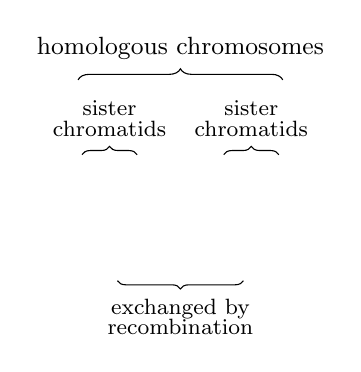
\begin{tikzpicture}[every node/.style={font=\small}]
      \chrom{0}{3}{0/1/red!60}\chrom{0.4}{3}{0/0.65/red!60,0.65/1/blue!50}
      \chrom{1.8}{3}{0/0.65/blue!50,0.65/1/red!60}\chrom{2.2}{3}{0/1/blue!50}
      \draw[decorate, decoration={brace, amplitude=3pt}] (-0.15,3.1) -- (0.55,3.1) node[midway, above=3pt, align=center, font=\footnotesize] {sister\\[-2pt]chromatids};
      \draw[decorate, decoration={brace, amplitude=3pt}] (1.65,3.1) -- (2.35,3.1) node[midway, above=3pt, align=center, font=\footnotesize] {sister\\[-2pt]chromatids};
      \draw[decorate, decoration={brace, amplitude=4pt}] (-0.2,4.05) -- (2.4,4.05) node[midway, above=4pt] {homologous chromosomes};
      \draw[decorate, decoration={brace, amplitude=3pt, mirror}] (0.3,1.5) -- (1.9,1.5) node[midway, below=3pt, align=center, font=\footnotesize] {exchanged by\\[-2pt]recombination};
    \end{tikzpicture}
    \caption{}
  \end{subfigure}
  \caption{(a) Inheritance through a pedigree (squares male, circles female). Each grandparent's two copies of one chromosome are given distinct colours. A parent passes on a mosaic of their two copies, so the child's paternal copy contains segments from both paternal grandparents. (b) Crossing over in meiosis. Each homologous chromosome (red, inherited from one parent; blue, from the other) is duplicated into two sister chromatids, and segments are exchanged between non-sister chromatids. Each resulting gamete receives one of the four chromatids.}
  \label{fig:recomb}
\end{figure}

Recombination is not uniform along the genome. In humans and many other mammals, most crossovers occur in \emph{recombination hotspots}, short regions of a few kilobases~\citep{myers2005}. Their positions are set largely by the zinc-finger protein PRDM9, which binds a specific DNA motif and marks nearby sites for recombination~\citep{baudat2010}. Dogs have lost a functional \textit{PRDM9} and lack such hotspots~\citep{axelsson2012}, and a woman with no functional PRDM9 was found to be healthy and fertile, with the crossovers in her children placed away from the usual hotspots~\citep{narasimhan2016}.

\subsection{Linkage disequilibrium}

Recombination is the reason that variants close together on a chromosome are correlated in a population. When a new mutation arises, it does so on one copy of the genome, alongside the particular alleles that copy carries at nearby SNPs. Over the following generations, recombination events between the mutation and a nearby SNP gradually break up this association, but if the two are close, a recombination between them is rare and the association persists for many generations. The non-random association of alleles at different loci is called \emph{linkage disequilibrium} (LD).

To quantify LD, consider two bi-allelic loci with alleles A/a and B/b, and let $f_A$ and $f_B$ be the frequencies of alleles A and B and $f_{AB}$ the frequency of haplotypes (single chromosome copies) carrying both A and B. If the loci were independent we would have $f_{AB}=f_Af_B$. The deviation
\begin{equation}
  D = f_{AB}-f_Af_B
\end{equation}
measures LD. Let $h_A\in\{0,1\}$ and $h_B\in\{0,1\}$ indicate whether a randomly chosen haplotype carries A and B. Then $\Cov(h_A,h_B)=\E[h_Ah_B]-\E[h_A]\E[h_B]=f_{AB}-f_Af_B=D$, and the squared correlation
\begin{equation}
  r^2 = \frac{D^2}{f_A(1-f_A)\,f_B(1-f_B)}
  \label{eq:r2}
\end{equation}
is the most widely used measure of LD. It lies between 0 (independence) and 1 (one allele perfectly predicts the other). The correlation between the dosages of two SNPs across individuals is approximately $r$ as well.

\paragraph{Decay of LD.} Let $c$ be the probability that a recombination occurs between the two loci in one meiosis, the \emph{recombination fraction}. Assume random mating in a large population and no selection. A haplotype in the next generation is non-recombinant with probability $1-c$, in which case it is a copy of a parental haplotype and carries A and B together with probability $f_{AB}$. With probability $c$ it is recombinant, its allele at the first locus comes from one parental haplotype and its allele at the second locus from the other, and in a randomly mating population these two haplotypes are independent, so it carries A and B with probability $f_Af_B$. Allele frequencies do not change, so the haplotype frequency and LD in the next generation are
\begin{align}
  f_{AB}' &= (1-c)f_{AB}+cf_Af_B,\\
  D' &= f_{AB}'-f_Af_B = (1-c)(f_{AB}-f_Af_B) = (1-c)D,
\end{align}
and after $t$ generations
\begin{equation}
  D_t = (1-c)^tD_0 .
\end{equation}
LD decays geometrically, at a rate set by the recombination fraction. For loci a few kilobases apart $c$ is of the order of $10^{-5}$ to $10^{-4}$, so LD can persist for thousands of generations. Recombination hotspots break LD sharply, so the genome is broken into \emph{LD blocks}, runs of SNPs with high mutual correlation separated by hotspots~\citep{gabriel2002}.

Random genetic drift in a finite population works in the opposite direction, creating LD by chance. The balance between the two depends on the effective population size and on the population's history. All modern humans descend from populations in Africa, and the ancestors of non-African populations left Africa around 60{,}000 years ago in a relatively small group that then expanded rapidly. This bottleneck means that non-African populations descend from fewer ancestral haplotypes and have had fewer generations of large population size, so LD extends further in non-African populations than in African populations~\citep{hapmap2005}, and African populations retain more genetic diversity than the rest of the world. Figure~\ref{fig:ld_heatmap} illustrates the effect in a simulation. A practical consequence is that association signals in African-ancestry cohorts are confined to fewer correlated SNPs, which helps to locate causal variants; most GWAS to date, however, have been in European-ancestry cohorts.

\begin{figure}[!htbp]
  \centering
  \includegraphics[width=0.9\linewidth]{ld_heatmap.pdf}
  \caption{Linkage disequilibrium ($r^2$ between pairs of SNPs, upper triangle) in two simulated populations of 1000 individuals that share recombination hotspots (triangles on the diagonal). Haplotypes were simulated as mosaics of ancestral founder haplotypes, switching founder rarely within blocks and often at hotspots. Left, a large population descended from 60 founder haplotypes with frequent historical recombination. Right, a population descended from 5 of the same founders with fewer generations of recombination, as after a bottleneck: LD is stronger and extends across blocks. SNPs with minor allele frequency above 5\% in both populations are shown in genomic order.}
  \label{fig:ld_heatmap}
\end{figure}

\subsection{LD and the causal variant}

LD is what makes a GWAS work with a few hundred thousand genotyped SNPs, since an untyped causal variant is detected through the typed SNPs correlated with it. It is also what makes it hard to tell which variant is causal. Figure~\ref{fig:fto_locus}A shows a \emph{LocusZoom} plot~\citep{pruim2010} of the strongest association with body mass index (BMI), in an intron of the gene \textit{FTO} on chromosome 16~\citep{frayling2007}. Each point is a SNP, placed by position and $-\log_{10}p$, and coloured by its $r^2$ with the most significant (lead) SNP. The blue line is the recombination rate, which peaks at two hotspots about 50 kb apart. Between them is an LD block of dozens of SNPs with p-values near $10^{-60}$, any of which could be causal. Panels B and C of the figure show how additional data can help, and we return to them in Section~\ref{sec:fto}.

\begin{figure}[!htbp]
  \centering
  \includegraphics[width=0.62\linewidth]{slides/fto_locus.png}
  \caption{The \textit{FTO} obesity locus. (A) LocusZoom plot of association with BMI; colour shows LD ($r^2$) with the lead SNP in European-ancestry (CEU) reference data, and the blue line the recombination rate. (B) Chromatin states inferred by ChromHMM in 127 reference epigenomes grouped by tissue or cell type; yellow and orange states are enhancers. (C) Enhancer activity of five 10-kb segments of the locus, risk versus non-risk haplotype, in a luciferase reporter assay. Reproduced from \citet{claussnitzer2015}.}
  \label{fig:fto_locus}
\end{figure}

%======================================================================
\section{Genotyping arrays and imputation}
\label{sec:imputation}
%======================================================================

Whole-genome sequencing reads the genotype at every position, but most large GWAS cohorts were genotyped with arrays that measure 300{,}000--1{,}000{,}000 SNPs. LD makes it possible to predict, or \emph{impute}, the genotypes at the millions of SNPs that were not measured, using a \emph{reference panel} of sequenced individuals such as the 1000 Genomes Project~\citep{kg2015} (Figure~\ref{fig:imputation}).

\begin{figure}[!htbp]
  \centering
  \begin{tikzpicture}[every node/.style={font=\small}]
    \node (ref) at (0,0) {%
      \setlength{\tabcolsep}{3.5pt}\begin{tabular}{|cccccccccccc|}
        \hline
        0&0&1&1&1&0&0&1&0&1&1&0\\ \hline
        0&0&0&0&1&1&1&0&1&0&0&1\\ \hline
        1&1&1&1&0&0&0&1&0&0&0&0\\ \hline
        1&0&1&1&0&0&1&1&1&1&0&1\\ \hline
      \end{tabular}};
    \node (stu) at (0,-2.6) {%
      \setlength{\tabcolsep}{3.5pt}\begin{tabular}{cccccccccccc}
        1&\textcolor{red}{?}&\textcolor{red}{?}&2&\textcolor{red}{?}&0&\textcolor{red}{?}&\textcolor{red}{?}&1&\textcolor{red}{?}&\textcolor{red}{?}&1\\
        1&\textcolor{red}{?}&\textcolor{red}{?}&1&\textcolor{red}{?}&0&\textcolor{red}{?}&\textcolor{red}{?}&1&\textcolor{red}{?}&\textcolor{red}{?}&0\\
        0&\textcolor{red}{?}&\textcolor{red}{?}&1&\textcolor{red}{?}&1&\textcolor{red}{?}&\textcolor{red}{?}&2&\textcolor{red}{?}&\textcolor{red}{?}&1\\
        2&\textcolor{red}{?}&\textcolor{red}{?}&2&\textcolor{red}{?}&0&\textcolor{red}{?}&\textcolor{red}{?}&0&\textcolor{red}{?}&\textcolor{red}{?}&0\\
        1&\textcolor{red}{?}&\textcolor{red}{?}&\textcolor{red}{?}&\textcolor{red}{?}&1&\textcolor{red}{?}&\textcolor{red}{?}&1&\textcolor{red}{?}&\textcolor{red}{?}&2\\
      \end{tabular}};
    \draw[<->] ($(ref.south west)+(-0.3,-0.35)$) -- ($(ref.south east)+(0.3,-0.35)$) node[right] {genome};
    \draw[decorate, decoration={brace, amplitude=4pt}] ($(ref.north east)+(0.15,0)$) -- ($(ref.south east)+(0.15,0)$) node[midway, right=6pt, align=left] {reference haplotypes\\(sequenced panel)};
    \draw[decorate, decoration={brace, amplitude=4pt}] ($(stu.north east)+(0.15,0)$) -- ($(stu.south east)+(0.15,0)$) node[midway, right=6pt, align=left] {study genotypes\\(array; dosages 0/1/2)};
  \end{tikzpicture}
  \caption{The imputation problem. Reference haplotypes (top; 0 and 1 are the two alleles) are known at all SNPs. Study individuals (bottom) are genotyped at a subset of SNPs and their genotypes at the remaining SNPs (red question marks) are predicted from the reference panel using LD; missing calls at typed SNPs are filled in the same way. Adapted from a diagram on the IMPUTE2 website.}
  \label{fig:imputation}
\end{figure}

The simplest view of imputation is as a regression: for each untyped SNP, train a model in the reference panel that predicts its genotype from nearby typed SNPs, and apply it to the study individuals. The standard methods, such as IMPUTE2~\citep{howie2009}, instead use a hidden Markov model (Chapter 6) introduced by \citet{li2003}. Each haplotype of a study individual is modelled as a mosaic of the reference haplotypes, exactly as in the simulation of Figure~\ref{fig:ld_heatmap}. The hidden state at SNP $s$ is which reference haplotype is being copied. The transition probability of switching to another reference haplotype between adjacent SNPs increases with the genetic distance between them, mimicking historical recombination. The emission probability is close to 1 if the study allele matches the copied haplotype and small otherwise, allowing for mutation and genotyping error. The forward-backward algorithm gives the posterior probability of each genotype at each untyped SNP, and the imputed dosage is its posterior mean, $\E[x_{is}]=P(x_{is}=1)+2P(x_{is}=2)\in[0,2]$. These fractional dosages are used directly in the regression~\eqref{eq:gwas_snp}. Imputation accuracy is lower for rare variants, which are poorly tagged by typed SNPs, and when the reference panel does not match the ancestry of the study. Imputation matters for fine-mapping as well: a causal variant that is neither genotyped nor imputed can never be identified.

%======================================================================
\section{The genetic architecture of complex traits}
\label{sec:architecture}
%======================================================================

\subsection{Heritability and variance explained}

The \emph{heritability} $h^2$ of a trait is the fraction of its variance across individuals in a population that is explained by genetic differences. For a phenotype standardized to variance one, a single SNP with allele frequency $f_s$ and per-allele effect $\beta_s$ explains
\begin{equation}
  q_s^2 = \Var(\beta_sx_{is}) = \beta_s^2\Var(x_{is}) = 2f_s(1-f_s)\beta_s^2
  \label{eq:varexp}
\end{equation}
of the variance, using $\Var(x_{is})=2f_s(1-f_s)$ under Hardy--Weinberg equilibrium. The power to detect it depends on $Nq_s^2$. From Section~\ref{sec:gwas_model}, with standardized genotype and phenotype $\hat z_s\approx\sqrt N r_s$, and the sample correlation $r_s$ has mean approximately $\pm q_s$ and variance approximately $1/N$. Hence
\begin{equation}
  \E[\hat z_s^2]\approx 1+Nq_s^2,
\end{equation}
and $\hat z_s^2$ follows approximately a non-central $\chi^2_1$ distribution with non-centrality parameter (NCP) $Nq_s^2$. At $p<5\times10^{-8}$, that is $|\hat z_s|>5.45$, 80\% power requires an NCP of about 40. With $N=100{,}000$, this means $q_s^2\geq 4\times10^{-4}$: a SNP with $f_s=0.3$ needs $|\beta_s|\geq0.03$ phenotypic standard deviations per allele, while a SNP with $f_s=0.005$ needs $|\beta_s|\geq0.2$.

\subsection{Polygenicity}

One of the main findings of GWAS is that complex traits are highly \emph{polygenic}: they are affected by very many variants, each with a small effect. Before GWAS, many expected a typical disease to involve perhaps ten genes. The schizophrenia GWAS of the Psychiatric Genomics Consortium found 108 associated loci in 2014~\citep{ripke2014} and 287 in 2022 as the sample size grew~\citep{trubetskoy2022} (Figure~\ref{fig:scz-11}), and estimates of the total number of contributing variants are in the thousands. \citet{boyle2017} argued that gene regulatory networks are so densely connected that variants affecting the expression of almost any gene expressed in the relevant cell types will eventually have a small knock-on effect on the core genes of the trait. They called this the \emph{omnigenic} model.

\begin{figure}[!htbp]
  \centering
  \includegraphics[width=0.7\linewidth]{slides/scz_manhattan.png}
  \caption{Manhattan plot of a schizophrenia GWAS, with 287 genome-wide significant loci (index SNPs as green diamonds above the red line, $p=5\times10^{-8}$). Reproduced from \citet{trubetskoy2022}.}
  \label{fig:scz-11}
\end{figure}

\subsection{Effect size and allele frequency}

Among associated variants there is an inverse relationship between effect size and minor allele frequency (Figure~\ref{fig:or_maf}). Common variants have odds ratios close to 1, while the few low-frequency variants with MAF below 1\% that reach significance have odds ratios of 2 or more.

\begin{figure}[!htbp]
  \centering
  \includegraphics[width=0.7\linewidth]{slides/t2d_or_maf.png}
  \caption{Odds ratio per allele against minor allele frequency for 403 distinct association signals for type 2 diabetes, at previously reported and novel loci (stars, primary signals; circles, secondary signals). Reproduced from \citet{mahajan2018}.}
  \label{fig:or_maf}
\end{figure}

Two factors produce this pattern. The first is \emph{negative selection}. A variant that increases disease risk reduces, however slightly, its carriers' expected number of children, so natural selection acts to lower its frequency. Selection is more effective on variants with larger effects, which are therefore held at low frequency, while very rare variants are close to invisible to selection. A convenient model lets the variance of effect sizes depend on allele frequency,
\begin{equation}
  \Var(\beta_s\mid f_s)\propto\bigl[2f_s(1-f_s)\bigr]^{S},
\end{equation}
where $S\leq0$ measures the strength of the coupling: $S=0$ means effect sizes are independent of frequency, and $S=-1$ means each variant explains the same variance~\eqref{eq:varexp} on average whatever its frequency. Estimates for many human traits are negative~\citep{zeng2018}. Selection does not act on variants whose effects appear after reproductive age, which is one reason that strong risk alleles for late-onset diseases, such as the $\varepsilon4$ allele of \textit{APOE} for Alzheimer's disease, are common.

The second factor is \emph{power}. Since detection requires $2f_s(1-f_s)\beta_s^2$ to exceed a threshold, rare variants are detected only if their effects are large, whatever the underlying distribution of effects. Figure~\ref{fig:power_maf} separates the two factors in a simulation. Without selection, the discovered variants are almost all common. With $S=-1$, rare variants with large effects are frequent enough that many are discovered, and the discoveries show a strong inverse relationship. In both cases the discoveries lie just above the detection threshold.

\begin{figure}[!htbp]
  \centering
  \includegraphics[width=0.9\linewidth]{power_maf.pdf}
  \caption{Lines, the per-allele effect (in phenotypic standard deviations) needed for 80\% power at $p<5\times10^{-8}$ for three sample sizes $N$, from~\eqref{eq:varexp}. Points, variants discovered in a simulated GWAS of $N=100{,}000$ individuals for a trait with heritability $0.5$ spread over 5000 causal variants, with minor allele frequencies drawn from the neutral spectrum and effect variance proportional to $[2f(1-f)]^S$. Left, no coupling between effect size and frequency ($S=0$): 524 variants are discovered, none with MAF below 1\%. Right, negative selection ($S=-1$): 545 discoveries, 267 with MAF below 1\%.}
  \label{fig:power_maf}
\end{figure}

%======================================================================
\section{Population structure and relatedness}
\label{sec:popstruct-11}
%======================================================================

\subsection{Confounding by ancestry}

The regression~\eqref{eq:gwas_snp} assumes independent noise. Two features of real samples violate this. The first is \emph{population structure} or \emph{stratification}: the sample contains people of different ancestry, allele frequencies differ by ancestry, and so does the phenotype, for genetic or environmental reasons. Then every SNP whose frequency differs between ancestry groups is associated with the phenotype, causal or not. A classic example comes from the Pima and Tohono O'odham communities of Arizona, where a haplotype of the immunoglobulin gene region \textit{Gm} was associated with lower risk of type 2 diabetes. The haplotype is common in Europeans and marked European admixture, which was itself associated with lower diabetes risk; within groups with the same degree of admixture the association disappeared~\citep{knowler1988}.

The second is \emph{relatedness}. Relatives share more of their genomes than unrelated people, and, for a heritable trait, more of their genetic predisposition. Unknown relatives in a sample (\emph{cryptic relatedness}) make the noise in~\eqref{eq:gwas_snp} correlated, so test statistics are inflated even at SNPs with no effect. Related individuals can be removed, but in large biobanks that discards many samples.

A simple diagnostic is the \emph{genomic inflation factor}~\citep{devlin1999}
\begin{equation}
  \lambda_{GC} = \frac{\operatorname{median}_s\,\hat z_s^2}{0.455},
\end{equation}
where 0.455 is the median of the $\chi^2_1$ distribution, so $\lambda_{GC}\approx1$ if most SNPs are null and the tests are calibrated. Dividing all $\chi^2$ statistics by $\lambda_{GC}$ (\emph{genomic control}) is a crude correction. As we will see in Section~\ref{sec:ldsc}, polygenicity alone also gives $\lambda_{GC}>1$ in large studies, so inflation is not by itself evidence of confounding.

\subsection{Genotype principal components}

Chapter 8 showed that the top principal components (PCs) of the standardized genotype matrix capture ancestry; for Europeans the first two reproduce a map of Europe. Including the top PCs as covariates $\vc_i$ in~\eqref{eq:gwas_snp} removes the part of genotype and phenotype explained by broad ancestry gradients~\citep{price2006}. By the Frisch--Waugh theorem, this is equivalent to regressing both $\mX_{:s}$ and $\vy$ on the PCs and testing the residuals. PCs work well for continuous ancestry gradients but do not capture fine-scale structure or family relationships.

\subsection{Linear mixed models}

A linear mixed model (LMM) accounts for both structure and relatedness. Let $s$ index the SNP being tested, $\mC\in\R^{N\times Q}$ the covariate matrix (including a column of ones) with coefficients $\vgamma\in\R^Q$, and $\beta_s\in\R$ the effect of SNP $s$. The model is
\begin{equation}
  \underbrace{\vy}_{N\times1} = \underbrace{\mX_{:s}}_{N\times1}\underbrace{\beta_s}_{1\times1} + \mC\vgamma + \underbrace{\vu}_{N\times1} + \underbrace{\veps}_{N\times1},\qquad
  \vu\sim\Normal(\mathbf{0},\sigma_g^2\mK),\qquad \veps\sim\Normal(\mathbf{0},\sigma_e^2\mI),
  \label{eq:lmm}
\end{equation}
where $\vu$ is a \emph{random effect} with covariance proportional to a relatedness matrix $\mK\in\R^{N\times N}$, $\sigma_g^2$ is the genetic variance component and $\sigma_e^2$ the noise variance. The usual choice is the \emph{realized relatedness matrix}
\begin{equation}
  \mK = \frac1P\mZ\mZ^\top,
\end{equation}
where $\mZ\in\R^{N\times P}$ is the genotype matrix with each column standardized to mean zero and variance one. Entry $K_{ii'}=\frac1P\sum_jZ_{ij}Z_{i'j}$ is the average over SNPs of the product of the two individuals' standardized genotypes. It is close to 1 for $i=i'$ and for identical twins, about $1/2$ for parents and children or siblings, $1/8$ for first cousins and near 0 for unrelated people. It is called ``realized'' because it estimates the relatedness actually realized in the genotypes rather than the relatedness expected from a pedigree. People of similar ancestry also have larger $K_{ii'}$, because they tend to share the alleles that are common in their ancestry group, so $\mK$ captures population structure too.

There is a useful interpretation of the random effect. Suppose all $P$ SNPs affect the trait, $\vu=\mZ\boldsymbol{\alpha}$, with independent effects $\alpha_j\sim\Normal(0,\sigma_g^2/P)$. Then $\Cov(\vu)=\mZ\,(\sigma_g^2/P)\mI\,\mZ^\top=\sigma_g^2\mK$. The LMM is therefore a joint regression on all SNPs with a Gaussian prior on their effects, which is ridge regression (Chapter 1), combined with a fixed effect for the SNP under test. Under this model $\sigma_g^2/(\sigma_g^2+\sigma_e^2)$ is the heritability explained by the SNPs~\citep{yang2010}. The background polygenic effect $\vu$ absorbs the phenotypic similarity of relatives and of people with shared ancestry, so it is not attributed to the test SNP.

\paragraph{Likelihood.} Integrating out $\vu$ and $\veps$, which are independent and Gaussian,
\begin{equation}
  \vy\sim\Normal\bigl(\mA\vtheta,\ \sigma_g^2\mK+\sigma_e^2\mI\bigr) = \Normal\bigl(\mA\vtheta,\ \sigma_g^2\mH\bigr),\qquad \mH=\mK+\delta\mI,
\end{equation}
where $\mA=[\mC,\mX_{:s}]\in\R^{N\times(Q+1)}$ collects the fixed-effect covariates, $\vtheta=(\vgamma^\top,\beta_s)^\top\in\R^{Q+1}$, and $\delta=\sigma_e^2/\sigma_g^2$. The log likelihood is
\begin{equation}
  \log L(\vtheta,\sigma_g^2,\delta) = -\frac N2\log(2\pi\sigma_g^2) - \frac12\log|\mH| - \frac1{2\sigma_g^2}(\vy-\mA\vtheta)^\top\mH^{-1}(\vy-\mA\vtheta).
  \label{eq:lmm_ll}
\end{equation}
For fixed $\delta$, setting the gradient with respect to $\vtheta$ to zero gives the generalized least squares (GLS) estimate, and setting the derivative with respect to $\sigma_g^2$ to zero gives its maximum likelihood estimate:
\begin{equation}
  \hat\vtheta = (\mA^\top\mH^{-1}\mA)^{-1}\mA^\top\mH^{-1}\vy,\qquad
  \hat\sigma_g^2 = \frac1N(\vy-\mA\hat\vtheta)^\top\mH^{-1}(\vy-\mA\hat\vtheta).
\end{equation}
Since $\hat\vtheta$ is linear in $\vy$, its covariance is $\Cov(\hat\vtheta)=\sigma_g^2(\mA^\top\mH^{-1}\mA)^{-1}$, and the test statistic for SNP $s$ is $\hat z_s=\hat\beta_s/\sqrt{\hat\sigma_g^2[(\mA^\top\mH^{-1}\mA)^{-1}]_{Q+1,Q+1}}$. Substituting $\hat\vtheta$ and $\hat\sigma_g^2$ into~\eqref{eq:lmm_ll} gives the profile log likelihood of $\delta$,
\begin{equation}
  \log L(\delta) = -\frac N2\bigl[\log(2\pi\hat\sigma_g^2(\delta))+1\bigr] - \frac12\log|\mK+\delta\mI|,
\end{equation}
a function of one scalar that can be maximized by a grid or line search.

\paragraph{Computation.} Evaluated naively, $\mH^{-1}$ and $\log|\mH|$ cost $O(N^3)$, for each value of $\delta$ and each of millions of SNPs, which is infeasible for $N$ in the hundreds of thousands. Two observations make LMMs practical. First, each SNP explains a tiny fraction of the variance, so $\delta$ can be estimated once under the null model without any test SNP and reused for all SNPs~\citep{kang2010}. Second, the eigendecomposition of $\mK$ diagonalizes $\mH$ for every $\delta$~\citep{lippert2011}. Write $\mK=\mU\mS\mU^\top$ with $\mU\in\R^{N\times N}$ orthogonal and $\mS=\operatorname{diag}(s_1,\dots,s_N)$ the eigenvalues. Then
\begin{equation}
  \mH = \mU(\mS+\delta\mI)\mU^\top,\qquad \mH^{-1}=\mU(\mS+\delta\mI)^{-1}\mU^\top,\qquad \log|\mH|=\sum_{i=1}^N\log(s_i+\delta).
\end{equation}
Define rotated data $\tilde\vy=\mU^\top\vy$ and $\tilde\mA=\mU^\top\mA$, with rows $\tilde\va_i^\top$. The quadratic form in~\eqref{eq:lmm_ll} becomes
\begin{equation}
  (\vy-\mA\vtheta)^\top\mH^{-1}(\vy-\mA\vtheta) = (\tilde\vy-\tilde\mA\vtheta)^\top(\mS+\delta\mI)^{-1}(\tilde\vy-\tilde\mA\vtheta) = \sum_{i=1}^N\frac{(\tilde y_i-\tilde\va_i^\top\vtheta)^2}{s_i+\delta},
\end{equation}
so in the rotated coordinates the LMM is a weighted least squares problem with independent observations and weights $1/(s_i+\delta)$. The eigendecomposition costs $O(N^3)$ once (or $O(NP_K^2)$ via a singular value decomposition of $\mZ$ if $\mK$ is built from $P_K<N$ SNPs). After that, each test SNP requires one rotation $\mU^\top\mX_{:s}$, which costs $O(N^2)$, or $O(NP_K)$ in the low-rank case, followed by $O(N)$ work. Methods for biobank-scale data, such as BOLT-LMM, avoid forming $\mK$ altogether by using iterative solvers~\citep{loh2015}.

Two practical points. If the test SNP, or SNPs in LD with it, are included in $\mK$, part of its effect is absorbed by $\vu$ and power is lost (\emph{proximal contamination}). The usual fix is to compute $\mK$ from all chromosomes except the one containing the test SNP (\emph{leave one chromosome out}). And the LMM is derived for a continuous trait; for case-control traits with strong ascertainment it remains widely used but needs care~\citep{yang2014}.

Figure~\ref{fig:popstrat} compares the three approaches in a simulation with two populations and sibling pairs. Plain regression is badly inflated at null SNPs. Adding two PCs removes most of the inflation, which comes from the population difference, but not the remainder due to relatedness. The LMM is close to calibrated.

\begin{figure}[!htbp]
  \centering
  \includegraphics[width=0.55\linewidth]{popstrat_qq.pdf}
  \caption{Quantile-quantile plot of p-values at 3000 null SNPs in a simulated cohort of 1000 people from two populations ($F_{ST}=0.01$), 60\% of them in sibling pairs. The phenotype has heritability 0.5 from 500 causal SNPs elsewhere in the genome, plus a non-genetic difference between the populations. Points above the dashed diagonal indicate inflated test statistics. The relatedness matrix $\mK$ for the LMM and the PCs were computed from 5000 SNPs that exclude the tested SNPs, as in leave-one-chromosome-out analysis.}
  \label{fig:popstrat}
\end{figure}

%======================================================================
\section{Summary statistics}
\label{sec:sumstats}
%======================================================================

\subsection{What and why}

A GWAS is usually reported as \emph{summary statistics}: for every SNP, the estimated effect $\hat\beta_s$, its standard error, the p-value, the alleles and their frequency, and the sample size. Any two of $\hat\beta_s$, $\operatorname{SE}(\hat\beta_s)$, $\hat z_s$ and the p-value (with the sign of the effect) determine the others approximately. Summary statistics have become the main currency of human genetics, for two reasons.
\begin{itemize}
  \item \emph{Sharing.} Individual genotypes and phenotypes are protected by the consent agreements under which they were collected and often cannot leave the institution or country that holds them. Summary statistics usually can be shared and are often public.
  \item \emph{Scale.} Individual-level data for a large GWAS is a matrix of millions of SNPs by hundreds of thousands of people. Summary statistics are a few numbers per SNP.
\end{itemize}
Sharing summary statistics allows \emph{meta-analysis}, combining studies of the same trait in different cohorts. In machine learning terms this is the simplest instance of federated learning, in which models are fitted where the data live and only parameters are pooled. Suppose $K$ cohorts report estimates $\hat\beta_{sk}$ with standard errors $\operatorname{SE}_{sk}$ for the same SNP $s$ and the same true effect $\beta_s$, $k=1,\dots,K$, so that $\hat\beta_{sk}\sim\Normal(\beta_s,\operatorname{SE}_{sk}^2)$ independently. The log likelihood of $\beta_s$ is $-\sum_k(\hat\beta_{sk}-\beta_s)^2/(2\operatorname{SE}_{sk}^2)$ plus a constant, and setting its derivative to zero gives the inverse-variance weighted estimate
\begin{equation}
  \hat\beta_s = \frac{\sum_kw_k\hat\beta_{sk}}{\sum_kw_k},\qquad w_k=\frac1{\operatorname{SE}_{sk}^2},\qquad \operatorname{SE}(\hat\beta_s)=\Bigl(\sum_kw_k\Bigr)^{-1/2}.
\end{equation}
This fixed-effects meta-analysis is what tools such as METAL implement~\citep{willer2010}. There is now a large literature of methods that use only summary statistics, often together with an estimate of the LD between SNPs from a reference panel~\citep{pasaniuc2017}.

\subsection{Summary statistics and LD}

Summary statistics together with the LD matrix carry essentially the same information as the individual-level data for a linear model. To see this, suppose that each column of $\mX\in\R^{N\times P}$ and $\vy$ are standardized to mean zero and variance one, where $\mX$ now holds the $P$ SNPs of one region, and that the phenotype follows a joint linear model in these SNPs,
\begin{equation}
  \vy=\mX\vb+\veps,\qquad\veps\sim\Normal(\mathbf{0},\sigma^2\mI),
\end{equation}
with true joint effects $\vb\in\R^P$. The noise $\veps$ includes the effects of variants elsewhere in the genome, which are unlinked to, and so uncorrelated with, the genotypes in the region. The per-SNP (marginal) least-squares estimate for SNP $j$ is $\hat\beta_j=\mX_{:j}^\top\vy/\mX_{:j}^\top\mX_{:j}=\mX_{:j}^\top\vy/N$. Stacking these into a vector,
\begin{equation}
  \hat\vb = \frac1N\mX^\top\vy = \frac1N\mX^\top\mX\vb + \frac1N\mX^\top\veps = \mR\vb + \frac1N\mX^\top\veps,
\end{equation}
where $\mR=\mX^\top\mX/N\in\R^{P\times P}$ is the matrix of correlations between SNPs, the \emph{LD matrix}, with ones on the diagonal and $R_{jk}=r_{jk}$. Given $\mX$, the noise term has mean zero and covariance $\frac1{N^2}\mX^\top(\sigma^2\mI)\mX=\frac{\sigma^2}N\mR$, so
\begin{equation}
  \hat\vb\sim\Normal\Bigl(\mR\vb,\ \frac{\sigma^2}N\mR\Bigr).
\end{equation}
A single region explains a small fraction of the phenotypic variance, so $\sigma^2\approx1$ and the marginal standard errors are all approximately $\sqrt{1/N}$. Defining the z-scores $\vzh=\sqrt N\hat\vb\in\R^P$ and the \emph{true} (joint) z-scores $\vz=\sqrt N\vb\in\R^P$,
\begin{equation}
  \vzh\sim\Normal(\mR\vz,\ \mR).
  \label{eq:zR}
\end{equation}
The true z-scores are unobserved. One way to think of them is as the expected z-score each SNP would have if it were the only SNP in the model, or, divided by $\sqrt N$, as the joint effect sizes that an infinitely large study would recover.

Equation~\eqref{eq:zR} says that the observed z-scores are the true z-scores \emph{mixed} by LD, plus noise that is itself correlated by LD. Suppose that a region contains a single causal SNP $c$, so that $\vz=z_c\ve_c$, where $\ve_c$ is the $c$-th standard basis vector. Then $\E[\hat z_j]=R_{jc}z_c$: the causal SNP has the largest expected signal, since $R_{cc}=1$, and the signal leaks into every SNP $j$ in proportion to its correlation with $c$. SNPs that are associated only through LD with a causal SNP are called \emph{tag} SNPs. The grey line in Figure~\ref{fig:finemap}a is this expected signal for a simulated locus. Because the noise is also correlated, a tag SNP can by chance have a larger $|\hat z_j|$ than the causal SNP.

Equation~\eqref{eq:zR} can be used as a likelihood, with $\vzh$ the observed data and $\vz$ latent variables to be inferred, and with priors on $\vz$ that may depend on features of each SNP~\citep{hormozdiari2014,zhu2017}. Two caveats apply. The derivation used the LD in the GWAS sample itself (\emph{in-sample} LD); in practice $\mR$ usually comes from a reference panel, and a mismatch between the two can create spurious signals. And $\mR$ is $P\times P$ with $P$ in the millions, but LD decays with distance, so $\mR$ is close to block diagonal and is stored and used one region at a time.

%======================================================================
\section{Fine-mapping}
\label{sec:finemap}
%======================================================================

\emph{Fine-mapping} is the task of identifying the causal variants within an associated locus, as opposed to the many tag SNPs. The usual approach is Bayesian: compute, for each SNP, the posterior probability that it is causal.

\subsection{A single causal variant}

Assume that a locus of $P$ SNPs contains exactly one causal SNP, with unknown index $c\in\{1,\dots,P\}$ and prior $P(c=j)=\pi_j$. Given $c=j$, the true z-scores are $\vz=\lambda\ve_j$, with $\lambda\sim\Normal(0,\omega^2)$ a prior on the causal effect on the z-score scale. Under the model~\eqref{eq:zR}, $\vzh\mid c=j,\lambda\sim\Normal(\lambda\vr_j,\mR)$, where $\vr_j$ is the $j$-th column of $\mR$.

The Bayes factor comparing ``SNP $j$ is causal'' with the null model $\vz=\mathbf{0}$ depends only on $\hat z_j$. To see this, factorize $p(\vzh)=p(\hat z_j)\,p(\vzh_{-j}\mid\hat z_j)$, where $\vzh_{-j}$ denotes the other $P-1$ z-scores. Under $c=j$, $\hat z_j\mid\lambda\sim\Normal(\lambda,1)$ since $R_{jj}=1$. By the conditioning formula for the multivariate Gaussian, the conditional distribution of the others is
\begin{equation}
  \vzh_{-j}\mid\hat z_j,\lambda\sim\Normal\bigl(\lambda\vr_{-j}+\vr_{-j}(\hat z_j-\lambda),\ \mR_{-j,-j}-\vr_{-j}\vr_{-j}^\top\bigr) = \Normal\bigl(\vr_{-j}\hat z_j,\ \mR_{-j,-j}-\vr_{-j}\vr_{-j}^\top\bigr),
\end{equation}
where $\vr_{-j}$ is $\vr_j$ without its $j$-th entry and $\mR_{-j,-j}$ is $\mR$ without row and column $j$. This does not depend on $\lambda$, and it is the same under the null ($\lambda=0$). It therefore cancels in the Bayes factor. Integrating $\lambda$ out of $p(\hat z_j\mid\lambda)$ gives $\hat z_j\sim\Normal(0,1+\omega^2)$ under $c=j$, against $\Normal(0,1)$ under the null, so
\begin{equation}
  \mathrm{BF}_j = \frac{\Normal(\hat z_j;0,1+\omega^2)}{\Normal(\hat z_j;0,1)} = \frac1{\sqrt{1+\omega^2}}\exp\left(\frac{\hat z_j^2}2\,\frac{\omega^2}{1+\omega^2}\right).
  \label{eq:abf}
\end{equation}
This is the approximate Bayes factor of \citet{wakefield2009}, written on the z-score scale: with $\hat\beta_j\sim\Normal(\beta_j,V)$ and prior $\beta_j\sim\Normal(0,W)$, $\omega^2=W/V$. The posterior probability that SNP $j$ is the causal one, its \emph{posterior inclusion probability} (PIP), follows from Bayes' rule:
\begin{equation}
  \mathrm{PIP}_j = P(c=j\mid\vzh) = \frac{\pi_j\mathrm{BF}_j}{\sum_{k=1}^P\pi_k\mathrm{BF}_k}.
  \label{eq:pip}
\end{equation}
A $95\%$ \emph{credible set} is the smallest set of SNPs whose PIPs sum to at least $0.95$~\citep{maller2012}. The single-causal-variant model needs only the marginal z-scores, not $\mR$. Its weakness is the assumption itself: many loci contain several independent signals. Models with multiple causal variants use $\mR$ explicitly, either by enumerating configurations of causal SNPs~\citep{hormozdiari2014} or, in the widely used SuSiE method, by writing $\vb$ as a sum of single-effect vectors, each of which has a single-causal-variant posterior of the form~\eqref{eq:pip}~\citep{wang2020susie}.

\subsection{Functional fine-mapping}

The prior $\pi_j$ need not be uniform. SNPs in regulatory elements of a relevant cell type, or SNPs that change protein sequence, are more likely to be causal. \emph{Functional fine-mapping} sets the prior from annotations of each SNP, for example
\begin{equation}
  \pi_j = \frac{\exp(\vlambda^\top\va_j)}{\sum_{k=1}^P\exp(\vlambda^\top\va_k)},
  \label{eq:annot_prior}
\end{equation}
a softmax over a linear function of an annotation vector $\va_j\in\R^L$ (for example, indicators of the ChromHMM state the SNP falls in, Chapter 6), with weights $\vlambda\in\R^L$. The weights are shared across many loci and learned by maximizing the marginal likelihood across loci (Section~\ref{sec:interpret}). \citet{mahajan2018} fine-mapped type 2 diabetes loci using chromatin states from pancreatic islets, the cell type thought to drive much of the genetic risk. Incorporating the annotations raised the PIPs of variants in islet enhancers and promoters and lowered those of variants in heterochromatin (Figure~\ref{fig:t2d_finemap}).

\begin{figure}[!htbp]
  \centering
  \includegraphics[width=0.5\linewidth]{slides/t2d_functional_finemap.png}
  \caption{Posterior probability that each variant is causal at type 2 diabetes loci, with and without a prior informed by islet chromatin states (colour). Variants in enhancers and promoters move above the diagonal. Reproduced from \citet{mahajan2018}.}
  \label{fig:t2d_finemap}
\end{figure}

Figure~\ref{fig:finemap} shows statistical and functional fine-mapping in a simulated locus. The causal SNP is in an LD block with several others. In this realization, which we chose because it illustrates the point (in most simulations of this locus the lead SNP is the causal one), noise makes a tag SNP the lead SNP. With a uniform prior the causal SNP has PIP 0.23 and the lead SNP 0.50; the 95\% credible set contains five SNPs, including the causal one. With a prior that gives SNPs in annotated elements ten times the weight of others, the causal SNP's PIP rises to 0.71.

\begin{figure}[!htbp]
  \centering
  \includegraphics[width=0.9\linewidth]{finemap.pdf}
  \caption{Fine-mapping a simulated locus (5000 individuals, 220 SNPs, three recombination hotspots), with a single causal SNP (ringed) whose true z-score is 7. (a) Marginal association, coloured by $r^2$ with the lead SNP; the grey line is the expected signal $-\log_{10}p$ of $R_{jc}z_c$, showing how the causal signal leaks into correlated SNPs. (b) Posterior inclusion probabilities with a uniform prior, using the Bayes factor~\eqref{eq:abf} with $\omega^2=112.5$. (c) PIPs with prior weight ten times higher for SNPs in annotated elements (shaded), one of which contains the causal SNP.}
  \label{fig:finemap}
\end{figure}

%======================================================================
\section{LD score regression}
\label{sec:ldsc}
%======================================================================

LD score regression~\citep{bulik2015} uses the relation~\eqref{eq:zR} to estimate heritability, and to separate polygenic signal from confounding, using only summary statistics and LD.

\subsection{Derivation}

Take the joint model $\vy=\mX\vb+\veps$ with standardized genotypes and phenotype, and treat the effects as random: $\beta_k$ independent across SNPs with mean zero and variance $h^2/P$, so that the $P$ SNPs together explain heritability $h^2$. From the derivation of~\eqref{eq:zR}, $\vzh=\sqrt N\mR\vb+\ve$ with $\ve\sim\Normal(\mathbf{0},\mR)$ independent of $\vb$, so for SNP $j$
\begin{equation}
  \hat z_j = \sqrt N\sum_{k=1}^PR_{jk}\beta_k + e_j .
\end{equation}
The statistic $\chi^2_j=\hat z_j^2$ has expectation
\begin{equation}
  \E[\chi^2_j] = N\,\E\Bigl[\Bigl(\sum_kR_{jk}\beta_k\Bigr)^2\Bigr] + \E[e_j^2] = N\sum_kR_{jk}^2\Var(\beta_k) + 1 = \frac{Nh^2}P\,\ell_j + 1,
\end{equation}
where the cross term vanishes because $\vb$ and $\ve$ are independent with mean zero, $\E[\beta_k\beta_{k'}]=0$ for $k\neq k'$, $\E[e_j^2]=R_{jj}=1$, and
\begin{equation}
  \ell_j = \sum_{k=1}^P r_{jk}^2
\end{equation}
is the \emph{LD score} of SNP $j$: the sum of its squared correlations with all SNPs, including itself. Since LD is local, the sum is computed in a window around $j$ (1 centimorgan in the original method). Applying~\eqref{eq:zR} to the whole genome glosses over one detail. The noise variance is $1-h^2$ rather than 1, but chance in-sample correlations between unlinked SNPs, of order $1/\sqrt N$ each, add about $h^2$ to $\E[\chi^2_j]$ when summed over the genome, so the constant term is still close to 1. \citet{bulik2015} handle this by noting that a sample $r^2$ has expectation $r^2+(1-r^2)/N$. The intuition is that a SNP's $\chi^2$ collects signal from every causal variant it tags, in proportion to $r^2$, so under polygenicity SNPs with high LD scores have larger $\chi^2$ on average (Figure~\ref{fig:ldscore_schematic}).

\begin{figure}[!htbp]
  \centering
  \begin{tikzpicture}[every node/.style={font=\small}, >=Stealth]
    \draw[thick] (0,0) -- (10,0);
    \foreach \x in {0.6,1.4,2.2,3.0,3.8,5.0,6.2,7.0,7.8,8.6,9.4} \fill[gray] (\x,0) circle (2pt);
    \fill[black] (5.0,0) circle (3pt) node[below=3pt] {$j$};
    \foreach \x/\i/\h in {2.2/1/1.3, 6.2/2/0.6, 8.6/3/1.2}
      {\fill[red!70!black] (\x,0) circle (3pt); \node[below=3pt] at (\x,0) {$k=\i$};
       \draw[->, red!70!black, thick] (\x,0.1) .. controls (\x,\h) and (5.0,\h) .. (5.0,0.12);
       \node[red!70!black, above] at ({(\x+5.0)/2},{0.75*\h}) {$r_{j\i}^2$};}
    \node[above] at (5.0,1.75) {$\chi^2_j$ collects signal from every SNP $k$ in LD with $j$};
  \end{tikzpicture}
  \caption{Intuition for LD scores. The test statistic at SNP $j$ (black) includes signal from the causal SNPs $k$ it is correlated with (red), each weighted by $r_{jk}^2$. Under polygenicity every SNP has a small effect, so $\E[\chi_j^2]$ grows with $\ell_j=\sum_kr_{jk}^2$.}
  \label{fig:ldscore_schematic}
\end{figure}

Confounding by population structure or cryptic relatedness adds a bias term $\sqrt Nb_j$ to $\hat z_j$, where $b_j$ reflects the correlation between SNP $j$ and the confounder. Let $a=\E[b_j^2]$. Allele frequency differences between populations arise from genetic drift at each SNP and are not systematically larger at SNPs with high LD scores, so to a good approximation $a$ does not depend on $\ell_j$, giving
\begin{equation}
  \E[\chi^2_j] = \frac{Nh^2}P\,\ell_j + Na + 1 .
  \label{eq:ldsc}
\end{equation}
This is a linear regression of $\chi^2_j$ on $\ell_j$ across SNPs, with slope $Nh^2/P$ and intercept $1+Na$. The $\chi^2_j$ come from summary statistics, $N$ is known and $\ell_j$ is computed from a reference panel, so fitting the regression estimates $h^2$ from the slope and the amount of confounding from the intercept. Inflation due to polygenicity increases with LD score; inflation due to confounding does not. In practice the regression is weighted to account for the heteroskedasticity and correlation of the $\chi^2_j$, and standard errors are estimated with a block jackknife over the genome.

Figure~\ref{fig:ldsc} applies~\eqref{eq:ldsc} to simulated summary statistics. Without confounding, $\lambda_{GC}=1.56$ although there is no confounding at all, and LD score regression gives an intercept of 1.00 and recovers $h^2=0.5$. With population stratification, the intercept rises to 1.27 (the value implied by the simulation is 1.24) while the slope, and so the heritability estimate, changes little.

\begin{figure}[!htbp]
  \centering
  \includegraphics[width=0.6\linewidth]{ldsc.pdf}
  \caption{LD score regression on simulated summary statistics for 98{,}000 SNPs, $N=50{,}000$ and $h^2=0.5$, generated from $\vzh=\sqrt N\mR\vb+\ve$ with $\mR$ from simulated haplotypes in 4000 regions of varying LD. Points are mean $\chi^2$ in bins of LD score, lines the least-squares fits to all SNPs. Stratification was simulated by adding a term proportional to each SNP's allele frequency difference between two populations.}
  \label{fig:ldsc}
\end{figure}

\subsection{Stratified LD score regression}

The same argument partitions heritability by functional annotation~\citep{finucane2015}. Let $C_1,\dots,C_M$ be sets of SNPs defined by annotations (coding, promoter, enhancer in a given tissue, and so on), which may overlap, and let the variance of each effect depend on the annotations of its SNP,
\begin{equation}
  \beta_k\sim\Normal\Bigl(0,\ \sum_{c=1}^M\tau_c\ind[k\in C_c]\Bigr),
\end{equation}
where $\tau_c$ is the per-SNP contribution to heritability of annotation $c$. Repeating the derivation,
\begin{equation}
  \E[\chi^2_j] = N\sum_kR_{jk}^2\sum_c\tau_c\ind[k\in C_c] + Na+1 = N\sum_{c=1}^M\tau_c\,\ell(j,c) + Na + 1,\qquad \ell(j,c)=\sum_{k\in C_c}r_{jk}^2,
\end{equation}
where $\ell(j,c)$ is the LD score of SNP $j$ with respect to annotation $c$: how much of the signal that SNP $j$ picks up comes from SNPs in $C_c$. Fitting this multiple regression of $\chi^2_j$ on the $M$ annotation-specific LD scores estimates the $\tau_c$. The heritability in annotation $c$ is $h^2(C_c)=\sum_{k\in C_c}\Var(\beta_k)$, and its \emph{enrichment} is the fraction of heritability in $C_c$ divided by the fraction of SNPs in $C_c$. \citet{finucane2015} fitted a baseline model of several dozen annotations, including coding, UTR, promoter and enhancer regions and conserved sequence. Regions conserved across mammals, which contain about 2.6\% of common SNPs, were the most enriched, explaining about a third of the heritability averaged across traits. The model also gives a principled test of tissue specificity (Section~\ref{sec:interpret}).

A cross-trait version regresses the product $\hat z_{1j}\hat z_{2j}$ of z-scores for two traits on $\ell_j$ to estimate their \emph{genetic correlation}~\citep{bulik2015b}. Schizophrenia, bipolar disorder and major depression, for example, are genetically correlated: variants that raise risk for one tend to raise risk for the others.

%======================================================================
\section{Interpreting GWAS associations}
\label{sec:interpret}
%======================================================================

\subsection{Most associations are non-coding}

A variant that changes the amino acid sequence of a protein points directly at a gene and suggests a mechanism. Most GWAS associations, however, lie in introns or between genes~\citep{hindorff2009}, and presumably act by changing how much of a gene is expressed, when and where, or how it is spliced. This makes them harder to interpret: the variant, the cell type in which it acts and the gene it regulates are all unknown.

\citet{pickrell2014} estimated the contribution of different classes of variant by fitting a hierarchical model to the summary statistics of 18 traits. The genome is split into regions $k$, each containing a set $S_k$ of SNPs and assumed to contain at most one causal variant. The model has two levels. The prior probability $\Pi_k$ that region $k$ contains an association depends on region-level features $I_{kl}$ (such as gene density), and given an association, the probability $\pi_{ik}$ that SNP $i$ is the causal one depends on SNP-level annotations $I_{il}$ (such as falling in a coding exon or in a DNase I hypersensitive site in some cell type):
\begin{equation}
  \logit(\Pi_k)=\log\frac{\Pi_k}{1-\Pi_k} = \kappa+\sum_{l=1}^{L_1}\gamma_lI_{kl},\qquad
  \pi_{ik} = \frac{e^{x_i}}{\sum_{j\in S_k}e^{x_j}},\quad x_i=\sum_{l=1}^{L_2}\lambda_lI_{il},
\end{equation}
where $\kappa$ is an intercept, $\gamma_l$ are the coefficients of the $L_1$ region-level features and $\lambda_l$ those of the $L_2$ SNP-level annotations. The second level is the functional prior~\eqref{eq:annot_prior}. Which SNP is causal is never observed, so the model is fitted by maximizing the marginal likelihood. By the law of total probability, the probability of the data $\mathcal{D}_k$ in region $k$ is $(1-\Pi_k)\,p(\mathcal{D}_k\mid\text{null})+\Pi_k\sum_{i\in S_k}\pi_{ik}\,p(\mathcal{D}_k\mid\text{SNP $i$ causal})$. Dividing by $p(\mathcal{D}_k\mid\text{null})$, which does not depend on the parameters, and using the Bayes factors~\eqref{eq:abf} gives the likelihood relative to the null,
\begin{equation}
  L_k(\kappa,\vgamma,\vlambda) = (1-\Pi_k) + \Pi_k\sum_{i\in S_k}\pi_{ik}\mathrm{BF}_i,
\end{equation}
and the parameters maximize $\sum_k\log L_k$. Once fitted, the model gives each region's posterior probability of containing an association and each SNP's PIP, from which the fraction of associations attributable to coding variants follows. That fraction ranged from a few percent to about 20\% across traits (Figure~\ref{fig:pickrell}a): the large majority of the signal is non-coding.

\subsection{Which tissues?}

If a trait's heritability is concentrated in regulatory elements active in one tissue, that tissue is likely to be where the causal variants act. Stratified LD score regression tests this directly: add an annotation of the regulatory elements of one cell type (for example, regions marked by the enhancer-associated histone modifications H3K27ac or H3K4me1 in Roadmap Epigenomics data, Chapter 3) to the baseline model and test whether its coefficient $\tau_c$ is positive. Controlling for the baseline annotations matters, because regulatory elements in every tissue are enriched for heritability compared with the genome as a whole. Figure~\ref{fig:pickrell}b shows the results for ten groups of cell types~\citep{finucane2015}. Most make biological sense: central nervous system (CNS) elements for schizophrenia and bipolar disorder, immune cells for rheumatoid arthritis and Crohn's disease, connective tissue and bone for height, liver for HDL cholesterol. BMI is enriched in CNS, consistent with a role for appetite and behaviour, as are years of education and smoking. The \textit{FTO} example below shows that adipose tissue matters for BMI too.

\begin{figure}[!htbp]
  \centering
  \begin{subfigure}[b]{\linewidth}
    \centering
    \includegraphics[width=0.45\linewidth]{slides/coding_fraction.png}
    \caption{}
  \end{subfigure}\\[4pt]
  \begin{subfigure}[b]{\linewidth}
    \centering
    \includegraphics[width=0.85\linewidth]{slides/tissue_enrichment.png}
    \caption{}
  \end{subfigure}
  \caption{(a) Estimated proportion of association signals due to non-synonymous (coding) variants for 18 traits, with confidence intervals. Reproduced from \citet{pickrell2014}. (b) Enrichment of heritability in regulatory elements of ten groups of cell types, estimated by stratified LD score regression, for twelve traits. Bars are $-\log_{10}p$ for a positive coefficient $\tau_c$; dashed lines are multiple-testing thresholds. Reproduced from \citet{finucane2015}.}
  \label{fig:pickrell}
\end{figure}

\subsection{Other routes to interpretation}

Annotation overlap is one of several tools for interpreting GWAS loci. Sequence-to-function models such as those of Chapters 2 and 3 predict the effect of each variant on chromatin accessibility or expression, by in silico mutagenesis (Chapter 4), and these predictions can serve as annotations $\va_j$. Molecular quantitative trait loci, genetic associations with molecular phenotypes such as gene expression, connect variants to genes and cell types directly; they are the subject of the next chapter.

%======================================================================
\section{Case study: the \textit{FTO} obesity locus}
\label{sec:fto}
%======================================================================

The strongest common-variant association with obesity, in both adults~\citep{frayling2007} and children~\citep{bradfield2012}, lies in the first introns of the gene \textit{FTO} on chromosome 16 (Figure~\ref{fig:fto_locus}A). It is a typical GWAS locus: dozens of SNPs in strong LD, in a non-coding region, with several genes nearby. For years it was assumed that the variants act through \textit{FTO}, simply because they lie inside it. \citet{claussnitzer2015} worked through the locus systematically, using many of the ideas of this book, and the story is one of the clearest dissections of a GWAS association.

\paragraph{Cell type.} Chromatin states inferred by ChromHMM (Chapter 6) across 127 Roadmap reference epigenomes showed that the region of strongest association is in an enhancer state in mesenchymal cells, a class that includes adipocyte (fat cell) progenitors, and not in most other cell types (Figure~\ref{fig:fto_locus}B). In a luciferase reporter assay, which measures how strongly a DNA segment drives expression of a reporter gene, one 10-kb segment carrying the risk haplotype had more than twice the enhancer activity of the non-risk haplotype (Figure~\ref{fig:fto_locus}C).

\paragraph{Target genes.} The enhancer could regulate any gene within reach. Hi-C data (Chapter 3) showed long-range contacts in pre-adipocytes between the risk region and promoters up to about a megabase away (Figure~\ref{fig:fto_genes}c), consistent with earlier evidence of contacts with \textit{IRX3} in other cell types~\citep{smemo2014}. Comparing expression between people carrying the risk and non-risk genotypes, in pre-adipocytes, showed no difference for \textit{FTO} itself but higher expression of \textit{IRX3} and \textit{IRX5}, which lie about 0.5 and 1.2 Mb away (Figure~\ref{fig:fto_genes}b). The effect was specific to pre-adipocytes. The obvious culprit, \textit{FTO}, appears innocent here; in many other loci, though, the nearest gene is the causal one.

\begin{figure}[!htbp]
  \centering
  \begin{subfigure}[b]{\linewidth}
    \centering
    \includegraphics[width=0.85\linewidth]{slides/fto_region.png}
    \caption{}
  \end{subfigure}\\[2pt]
  \begin{subfigure}[b]{\linewidth}
    \centering
    \includegraphics[width=0.85\linewidth]{slides/fto_expression.png}
    \caption{}
  \end{subfigure}\\[2pt]
  \begin{subfigure}[b]{\linewidth}
    \centering
    \includegraphics[width=0.55\linewidth]{slides/fto_hic.png}
    \caption{}
  \end{subfigure}
  \caption{Target genes of the \textit{FTO} risk locus. (a) The 2.5-Mb region around the locus, with genes; points show LD with the lead SNP rs9930506 and the blue line the recombination rate. The LD block (grey) is confined to \textit{FTO}. (b) Expression of genes in the region in human pre-adipocytes from carriers of the risk and non-risk genotypes, with distance from the risk variant; only \textit{IRX3} and \textit{IRX5} differ. (c) LD (lower triangle, red) and Hi-C contact frequency in pre-adipocytes (upper triangle, blue) across the region; the risk variant rs1421085 contacts distant promoters although LD does not extend to them. Reproduced from \citet{claussnitzer2015}.}
  \label{fig:fto_genes}
\end{figure}

\paragraph{Causal variant and mechanism.} Using conservation and the predicted disruption of transcription factor binding motifs to prioritize among the SNPs in the block, \citet{claussnitzer2015} identified rs1421085 as the likely causal variant: its risk allele (C instead of T) disrupts a binding motif for the repressor ARID5B, derepressing the enhancer and raising \textit{IRX3} and \textit{IRX5} expression. Higher \textit{IRX3} and \textit{IRX5} expression shifts the fate of adipocyte progenitors away from \emph{beige} adipocytes, which burn lipids to produce heat (thermogenesis), toward \emph{white} adipocytes, which store lipids. Editing the risk allele to the non-risk allele with CRISPR-Cas9 in adipocyte progenitors from risk-allele carriers restored thermogenesis. A tendency to store rather than burn energy was probably advantageous when food was scarce and is maladaptive when it is abundant.

The \textit{FTO} story uses most of the steps that are now standard in interpreting a GWAS locus: fine-mapping within the LD block, chromatin state annotations to find the relevant cell type, chromatin contacts and expression differences between genotypes to find the target genes, sequence motifs to find the causal variant, and experiments to confirm the mechanism. It also suggests possible interventions, for example reducing \textit{IRX3} or \textit{IRX5} activity in adipocyte progenitors.

%======================================================================
\section{Summary}
%======================================================================

\begin{itemize}
  \item Humans differ at millions of sites, mostly SNPs. Most SNPs are rare, but most of the differences between two people are at common SNPs.
  \item Mendelian diseases are caused by variants in single genes; complex traits are influenced by thousands of variants of small effect together with environment. Large-effect variants tend to be rare, because of negative selection and because rare variants are detected only when their effects are large.
  \item A GWAS regresses the phenotype on each SNP's dosage separately and calls associations at $p<5\times10^{-8}$.
  \item Recombination breaks up the correlation between nearby variants slowly, $D_t=(1-c)^tD_0$, leaving LD blocks between hotspots. LD allows imputation of unmeasured SNPs from reference panels, with hidden Markov models, but makes the causal variant within a block hard to identify.
  \item Population structure and relatedness confound association tests. Genotype PCs correct for broad ancestry; linear mixed models with a realized relatedness matrix correct for both, and an eigendecomposition makes them fast.
  \item Summary statistics are easy to share and meta-analyse. Under a linear model, marginal z-scores satisfy $\vzh\sim\Normal(\mR\vz,\mR)$: the true signal is mixed by LD.
  \item Fine-mapping computes posterior inclusion probabilities and credible sets; under a single causal variant they depend only on the marginal z-scores. Functional annotations sharpen them through the prior.
  \item LD score regression, $\E[\chi^2_j]=Nh^2\ell_j/P+Na+1$, separates polygenicity (slope) from confounding (intercept), and its stratified form partitions heritability across annotations and tissues.
  \item Most associations are non-coding and act through gene regulation in specific cell types; finding the causal variant, cell type and gene, as at \textit{FTO}, remains the central task after a GWAS.
\end{itemize}

%======================================================================
\section*{Exercises}
%======================================================================

\begin{enumerate}
  \item Show that for two loci, $D=f_{AB}f_{ab}-f_{Ab}f_{aB}$, where the four terms are haplotype frequencies. If $c=0.01$, how many generations does it take for $D$ to halve?
  \item Under Hardy--Weinberg equilibrium, show that $\Var(x_{is})=2f_s(1-f_s)$. For $N=500{,}000$, what per-allele effect gives 80\% power at $p<5\times10^{-8}$ for a SNP with MAF 1\%? Use the non-centrality parameter of about 40.
  \item Derive the profile log likelihood of $\delta$ for the LMM by substituting $\hat\vtheta$ and $\hat\sigma_g^2$ into~\eqref{eq:lmm_ll}, and write it in terms of the eigenvalues of $\mK$ and the rotated data.
  \item Suppose a locus contains two SNPs with correlation $r$, one of which is causal with true z-score $z$. Using~\eqref{eq:zR}, find the probability that the non-causal SNP has the larger $|\hat z|$ as a function of $r$ and $z$, and evaluate it for $r=0.95$, $z=6$.
  \item Show that inverse-variance weighted meta-analysis of $K$ cohorts gives the same $\hat\beta$ as pooling the data into one regression when there are no covariates, the genotypes are centered within each cohort and the noise variance is the same in every cohort.
  \item Extend the LD score regression derivation to two traits measured in the same individuals, with genetic covariance $\rho_g$ between the effects $\beta_{1k}$ and $\beta_{2k}$ and phenotypic correlation $\rho$, and find $\E[\hat z_{1j}\hat z_{2j}]$.
  \item Implement the single-causal-variant fine-mapping of Section~\ref{sec:finemap}, apply it to the simulated locus in \texttt{make\_figures.py}, and study how the size of the 95\% credible set changes with $N$ and with the LD around the causal SNP.
\end{enumerate}
